
\subsection{Definition}

\textbf{Dynamic programming} is a method for solving a complex problem by breaking it down 
into a collection of simpler subproblems, \textbf{solving each of those subproblems just once, 
and storing their solutions in memory}. The next time the same subproblem occurs, instead of 
recomputing its solution, one simply looks up the previously computed solution, thereby 
\textbf{saving computation time at the expense of storage space}.

\subsection{Solving the knapsack problem with DP}

\subsubsection{The knapsack problem}

The knapsack problem is specified as follow : Given a set of item I, each item i being 
associated with a given value $(V_i)$ and weight $(W_i)$. Maximize the value of 
selected items. 

\begin{center}
\Large{$\sum_{i \in I} v_i x_i$}
\end{center}

Under constraint that the total capacity cannot exceed a given maximal capacity C 
and that an item cannot be partially selected. \newline

\begin{center}
\Large{$\sum_{i \in I} w_i x_i \le C$}

\vspace{3 mm}
\Large{$x_i \in \{0,1\}$}
\end{center}

Note that Knapsack is an NP-Complete problem as it can be used
to find a solution to the subset sum problem, which is NP-complete.

\begin{figure}[!ht]
	\centering
	\begin{framed}
	Given a set of natural number and a capacity K. 
	Find a subset S such that :\newline
	\Large{$\sum_{i \in S} c_i = K$}
	\end{framed}
	\caption{Subset sum problem}
\end{figure}
\FloatBarrier

\subsubsection{DP Solution for knapsack $\theta$(Cn)}

Let us refer to the optimal objective of the problem with capacity k and
items \{1,…,j\} $\in$ I as O(k,j). We can easily notice that :

\[ O(k,0) = 0 \]
\[ O(k,j) = \begin{cases} 
      max(O(k,j-1) , vj +O(k-wj,j-1))& if \quad wj \leq k \\
      O(k,j-1) & otherwise
   \end{cases}
\]

The goal of our knapsack problem can then be reduced to finding O(Cn) as shown in the 
following example :

\begin{figure}[!ht]
    \centering
    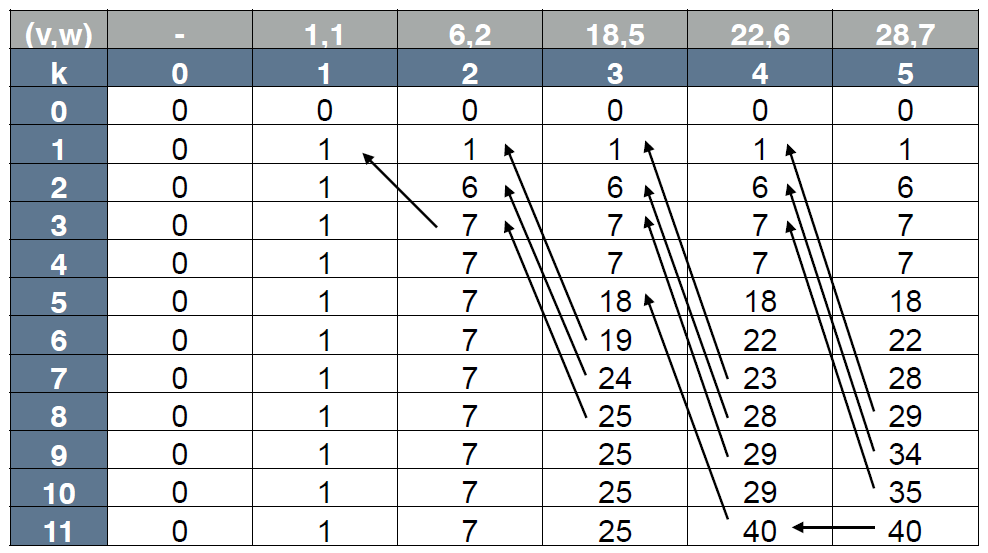
\includegraphics[width=0.7\linewidth]{KnapsackDP.png}
    \caption{Knapsack example}
    \label{fig:Knapsack_example}
\end{figure}
\FloatBarrier

\subsubsection{DP Solution for knapsack $\theta$(Vn)}

TODO


